% chktex-file 1
% chktex-file 2
% chktex-file 3
% chktex-file 8
% chktex-file 9
% chktex-file 12
% chktex-file 13
% chktex-file 16
% chktex-file 18
% chktex-file 24
% chktex-file 26
% chktex-file 35
% chktex-file 44
% chktex-file 45

\documentclass[]{article}
\usepackage[utf8]{inputenc}
\usepackage[english]{babel}

\usepackage[]{csvsimple}
\usepackage[]{float}

\usepackage{ragged2e}
\usepackage[left=25mm, right=25mm, top=15mm]{geometry}
\geometry{a4paper}
\usepackage{graphicx}
\usepackage{booktabs}
\usepackage{paralist}
\usepackage{subfig} 
\usepackage{fancyhdr}
\usepackage{amsmath}
\usepackage{amssymb}
\usepackage{amsfonts}
\usepackage{amsthm}
\usepackage{mathtools}
\usepackage{enumitem}
\usepackage{titlesec}
\usepackage{braket}
\usepackage{gensymb}
\usepackage{url}
\usepackage{hyperref}
\usepackage{csquotes}
\usepackage{multicol}
\usepackage{graphicx}
\usepackage{wrapfig}
\usepackage{babel}
\usepackage{caption}
\captionsetup{font=small}
\pagestyle{fancy}
\renewcommand{\headrulewidth}{0pt}
\lhead{}\chead{}\rhead{}
\lfoot{}\cfoot{\thepage}\rfoot{}
\usepackage{sectsty}
\usepackage[nottoc,notlof,notlot]{tocbibind}
\usepackage[titles,subfigure]{tocloft}
\renewcommand{\cftsecfont}{\rmfamily\mdseries\upshape}
\renewcommand{\cftsecpagefont}{\rmfamily\mdseries\upshape}

\let\oldsection\section% Store \section
\renewcommand{\section}{% Update \section
	\renewcommand{\theequation}{\thesection.\arabic{equation}}% Update equation number
	\oldsection}% Regular \section
\let\oldsubsection\subsection% Store \subsection
\renewcommand{\subsection}{% Update \subsection
	\renewcommand{\theequation}{\thesubsection.\arabic{equation}}% Update equation number
	\oldsubsection}% Regular \subsection

\newcommand{\abs}[1]{\left\lvert#1\right\rvert}
\newcommand{\norm}[1]{\left\lVert#1\right\rVert}

\newcommand{\g}{\text{g}}
\newcommand{\m}{\text{m}}
\newcommand{\cm}{\text{cm}}
\newcommand{\mm}{\text{mm}}
\newcommand{\s}{\text{s}}
\newcommand{\N}{\text{N}}
\newcommand{\Hz}{\text{Hz}}

\newcommand{\virgolette}[1]{``\text{#1}"}
\newcommand{\tildetext}{\raise.17ex\hbox{$\scriptstyle\mathtt{\sim}$}}


\renewcommand{\arraystretch}{1.2}

\addto\captionsenglish{\renewcommand{\figurename}{Fig.}}
\addto\captionsenglish{\renewcommand{\tablename}{Tab.}}

\DeclareCaptionLabelFormat{andtable}{#1~#2  \&  \tablename~\thetable}

\title{%
    \Huge Misura dell'indice di rifrazione di un vetro con lo spettrometro a prisma \\
    \Large Laboratorio di Ottica, Elettronica e Fisica Moderna \\ C.d.L. in Fisica, a.a. 2023-2024 \\ Università degli Studi di Milano}
\author{\LARGE Lucrezia Bioni, Leonardo Cerasi, Giulia Federica Bianca Coppi \\ Matricole: 13655A, 11410A, 11823A}
\date{23 novembre 2023}

\begin{document}

    \maketitle

    \section{Introduzione}

    \subsection{Scopo}

    Mediante l'utilizzo di un prisma a sezione isoscele, si vuole misurare l'indice di rifrazione del materiale che lo compone. Si vuole inoltre verificare la legge di dispersione secondo la formula di Cauchy:
    \begin{equation}
        \label{cauchy}
        n^2(\lambda) = A + \frac{B}{\lambda^2}
    \end{equation}
    dove dove $n$ è l'indice di rifrazione, $\lambda$ è la lunghezza d'onda, $A$ e $B$ sono dei coefficienti. Questi possono essere determinati per un materiale interpolando l'equazione ad indici di rifrazione misurati per lunghezze d'onda note.

    \subsection{Metodo}

    In seguito alla misurazione dello spettro di emissione della lampada ai vapori di mercurio - effettuata con il reticolo di diffrazione -, si utilizzano le lunghezze d'onda trovate per misurare l'indice di rifrazione del materiale vetroso che compone il prisma. \\
    Tale misurazione viene effettuata attraverso il metodo della deviazione minima: si può ricavare la dipendenza dell'angolo $\delta$ in funzione dell'angolo di incidenza $i$, dimostrando inoltre che la funzione $\delta (i)$ presenta un minimo. La condizione di deviazione minima si presenta nel momento in cui viene soddisfatta l'equazione:
    \begin{equation}
        \label{dev_minima}
        \cos i \cdot \cos r' = \cos r \cdot \cos i'
    \end{equation}
    dove $i$ è l'algolo di incidenza, $i'$ è l'angolo di emergenza, $r$ è l'angolo di rifrazione sulla faccia di entrata del prisma e $r'$ l'angolo di incidenza sulla seconda faccia del prisma.\\
    Queste quantità sono legate a $\delta$ dalle seguenti relazioni:
    \begin{equation}
        \label{relazioni_delta}
        r + r' = \alpha \qquad\qquad
        \delta = i + i' - \alpha
    \end{equation}
    dove $\alpha$ è l'angolo al vertice del prisma.\\
    L'indice di rifrazione del prisma, in condizioni di minima deviazione, risulterà essere quindi:
    \begin{equation}
        \label{indice_rifrazione}
        n(\lambda)=\frac{\sin \frac{\alpha + \delta _m} {2}}{\sin \frac{\alpha}{2}}
    \end{equation}
    dove $n(\lambda)$ è l'indice di rifrazione del materiale in funzione della lunghezza d'onda $\lambda$ considerata, $\alpha$ l'angolo al vertice della sezione del prisma, $\delta _m $ l'angolo di minima deviazione della lunghezza d'onda considerata.

    \section{Misure}
    \label{par:misure}

    \subsection{Angolo del prisma}
    Per misurare l'angolo $\alpha$ del prisma si sfrutta il fenomeno della riflessione: in particolare, si misurano le posizioni angolari $\theta_1$, $\theta_2$ delle immagini della fenditura riflesse da due facce consecutive del prisma. tramite un nonio sessagesimale di risoluzione $1'$. I dati sono riportati in Tab. \ref{theta-1-2-alpha}.

    \subsection{Angolo di deviazione minima}
    Per procede alla misura dell'angolo di deviazione minima, bisogna prima determinare la posizione angolare iniziale $\theta_0$ della fenditura in assenza di prisma: le misurazioni sono riportate in Tab. \ref{theta-0}. \\
    Una volta determinato $\theta_0$, si procede alla ricerca dell'angolo di deviazione minima per ciascuna lunghezza d'onda considerata: per fare ciò, si misura la posizione angolare $\theta_{\lambda}$ del punto di inversione del moto della riga spettrale considerata. I dati così ottenuti sono riportati in Tabb. \ref{viola-1} - \ref{giallo-2}.

    \section{Analisi dati}
    \subsection{Elaborazione dati}
    \subsubsection{Angolo del prisma}
    Dalla misura della posizione del fascio di luce riflessa da due delle facce del prisma, si ricava la posizione dell'angolo $\alpha$ compreso tra le due facce attraverso la seguente relazione:
    \begin{equation}
        \label{alpha}
        \alpha = 180\degree - \Delta\theta
    \end{equation}
    dove $\Delta\theta=\theta_2-\theta_1$, e $\theta_1$ è la posizione angolare del fascio riflesso dalla prima faccia, mentre $\theta_2$ è la posizione angolare del fascio riflesso dalla seconda.
    Tale calcolo è stato eseguito per ogni set di misure di $\theta_1$ e $\theta_2$ (vedere Tab. \ref{theta-1-2-alpha}), ed è stata effettuata una media aritmetica per determinare il valore finale di $\alpha$, pari a: 
    \begin{equation}
        \label{alpha-value}
        \alpha = 59 \degree \, 53' \pm 12'
    \end{equation}
    Dove l'errore è stato attribuito come da Par. \ref{par:alpha_err}.

    \subsubsection{Angolo di deviazione minima}
    Per determinare la posizione angolare $\theta_0$ del cannocchiale nella direzione da cui proviene l'immagine diretta della fenditura, si è eseguita la media aritmetica tra i valori di $\theta_0$ misurati (vedere Tab. \ref{theta-0}):
    \begin{equation}
        \label{theta-0-eq}
        \theta_0 = -(1 \degree \, 18' \, 0'' \pm 40'') 
    \end{equation}
    Per ciascuna lunghezza d'onda dello spettro del mercurio, si determina l'angolo di inversione $\delta$ del moto dell'immagine osservata mediante il cannocchiale attraverso la seguente relazione:
    \begin{equation}
        \label{delta}
        \delta = | \theta_0 - \theta_{\lambda}|
    \end{equation}
    dove $\theta_{\lambda}$ è la posizione angolare misurata del punto di inversione del moto (vedere Tabb. \ref{viola-1} - \ref{giallo-2}).
    Attraverso la media aritmetica dei valori di $\delta$ ottenuti, se ne determina la miglior stima: i valori ottenuti per ciascuna lunghezza d'onda osservata, con le loro incertezze (ricavate come da Par. \ref{par:dev_min_err}), sono riportati nella seguente tabella:
    \begin{table} [H]
        \centering
        \begin{tabular}{||c|c||}
            \hline
            Colore & $\delta \pm \sigma_{\delta}$\\
            \hline \hline
            Viola 1  & $ 74 \degree \,  9' \, 0'' \pm  1' \,  8'' $ \\\hline
            Viola 2  & $ 73 \degree \, 53' \, 0'' \pm  44'' $ \\\hline
            Indaco   & $ 71 \degree \, 47' \, 0'' \pm 27''         $ \\\hline
            Ciano    & $ 68 \degree \, 58' \, 0'' \pm  32'' $ \\\hline
            Verde    & $ 67 \degree \, 16' \, 0'' \pm   17'' $ \\\hline
            Giallo 1 & $ 66 \degree \, 33' \, 0'' \pm    14'' $ \\\hline
            Giallo 2 & $ 66 \degree \, 32' \, 0'' \pm        10'' $ \\\hline
        \end{tabular}
        \caption{Valori di $\delta$ e relativi errori.}
        \label{d-values}
    \end{table}

    \subsubsection{Indice di rifrazione del vetro}
    Ottenuti i valori dell'angolo di deviazione minima $\delta$ per ciascuna lunghezza d'onda e dell'angolo $\alpha$ al vertice del prisma, attraverso la relazione \ref{indice_rifrazione}, si ricavano i seguenti valori di indice di rifrazione del vetro del prisma $n$ in funzione della lunghezza d'onda $\lambda$:
    \begin{figure}[H]
        \centering
        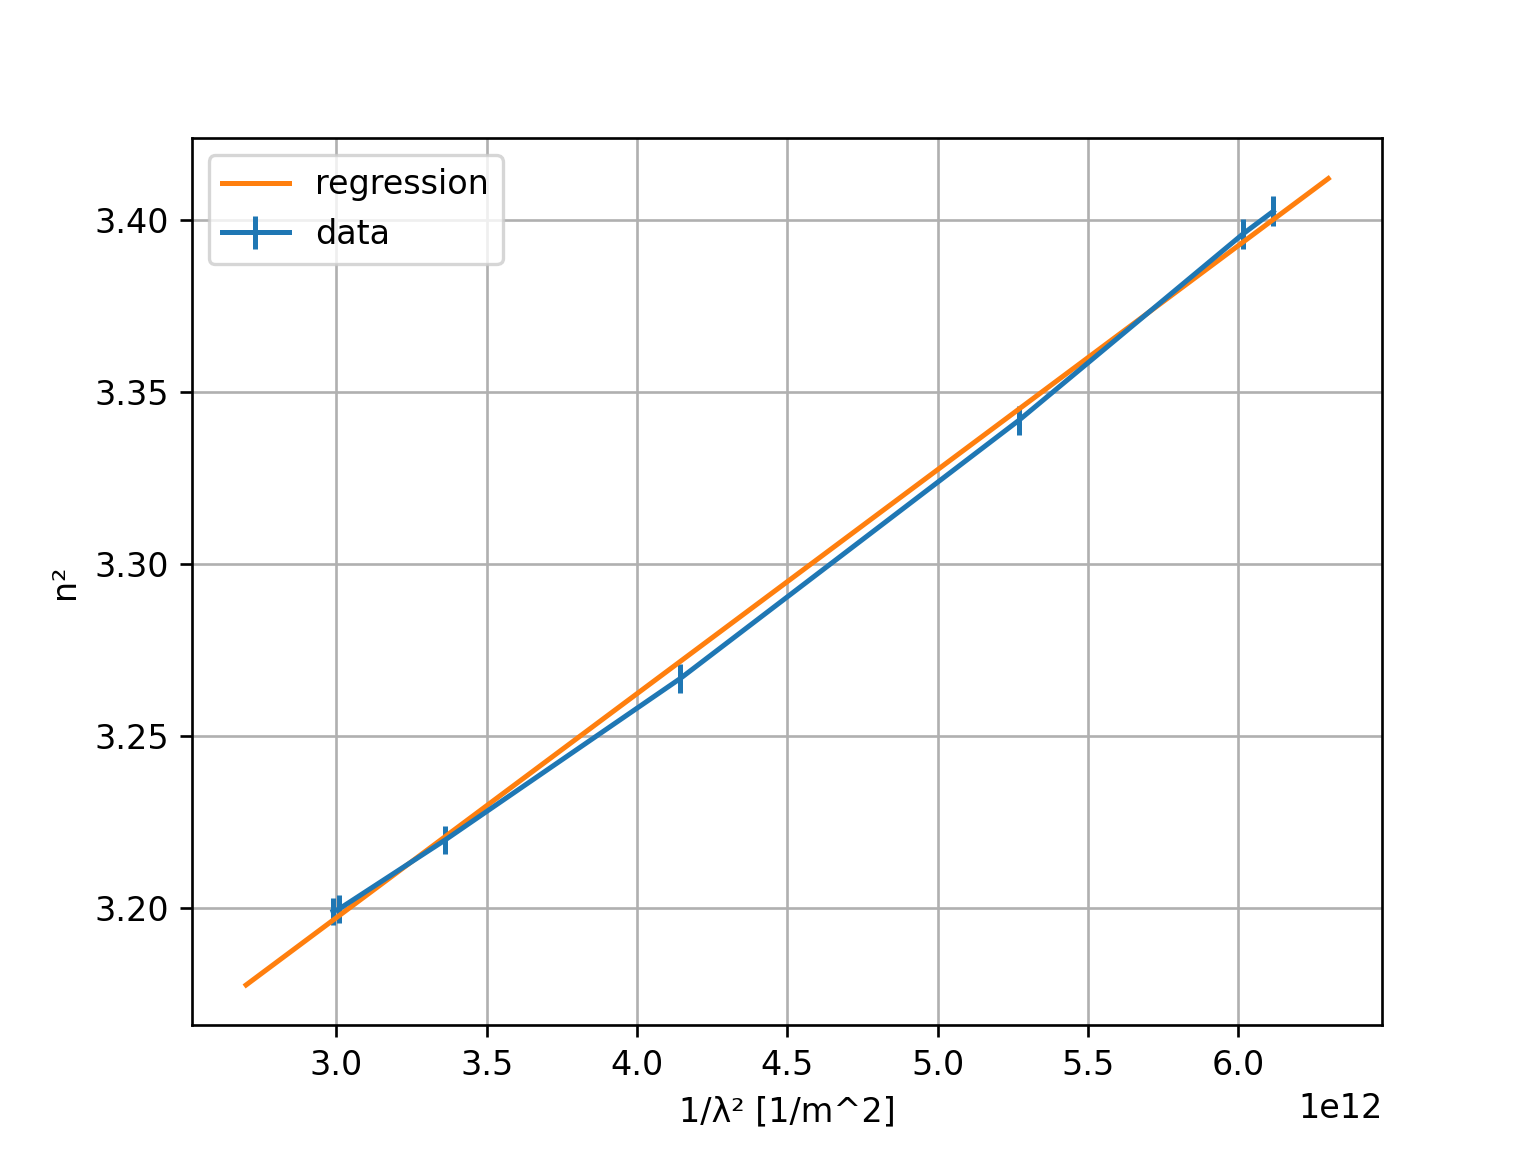
\includegraphics[width=0.40\textwidth]{graph/graph.png}
        \begin{tabular}[b]{||c|c|c||}
            \hline
            Colore & $\lambda \pm \sigma_{\lambda} \left[\text{nm}\right]$ & $ n(\lambda) \pm \sigma_n $\\
            \hline \hline
            Viola 1  & $404.32 \pm 0.08 $ & $1.845 \pm 0.004$ \\\hline
            Viola 2  & $407.70 \pm 0.10 $ & $1.843 \pm 0.004$ \\\hline
            Indaco   & $435.57 \pm 0.08 $ & $1.828 \pm 0.004$ \\\hline
            Ciano    & $491.21 \pm 0.08 $ & $1.807 \pm 0.004$ \\\hline
            Verde    & $545.44 \pm 0.08 $ & $1.794 \pm 0.004$ \\\hline
            Giallo 1 & $576.46 \pm 0.08 $ & $1.789 \pm 0.004$ \\\hline
            Giallo 2 & $578.41 \pm 0.08 $ & $1.789 \pm 0.004$ \\\hline
        \end{tabular}
        \captionlistentry[table]{Relazione di Cauchy.}
        \captionsetup{labelformat=andtable}
        \caption{Relazione di Cauchy.}
        \label{graph-cauchy}
    \end{figure}
    Per verificare la relazione di Cauchy \ref{cauchy}, sono stati riportati sul grafico i valori ottenuti dalle misure e dalla loro elaborazione. In particolare, si è posto sulle ascisse il termine $\frac{1}{\lambda^2}$ e sulle ordinate il valore $n^2$. Attraverso la regressione lineare pesata si sono ottenuti come valori del coefficiente angolare $A$ e del termine noto $B$ i seguenti:
    \begin{equation}
        \label{A}
        A = (3.002 \pm 0.006) 
    \end{equation}
    \begin{equation}
        \label{B}
        B = (6.5 \pm 0.1) \cdot 10^{-14} \text{m}^2
    \end{equation}
    Per verificare l'effettivo andamento lineare dei risultati ottenuti è stato effettuato un test del $\chi^2$:
    \begin{equation}
        \label{chi2}
        \chi^2 = 0.5623 
    \end{equation}
    Tale valore restituisce una compatibilità con un andamento lineare di probabilità $76.07 \% $.
    
    \subsection{Stima degli errori}
    \subsubsection{Angolo del prisma}
    L'errore attribuito ai singoli valori di $\alpha$ è stato ottenuto propagando l'errore su $\theta_1$ e $\theta_2$ nella \ref{alpha}:
    \begin{equation}
        \label{alpha-err}
        \sigma_{\alpha} = \sqrt{2} \cdot \sigma_{\theta} = 1' 25'' 
    \end{equation}
    Al valore finale di $\alpha$ è stata attribuita come incertezza la deviazione standard della media delle misure effettuate.
    \label{par:alpha_err}

    \subsubsection{Angolo di deviazione minima}
    L'errore attribuito al valore medio di $\theta_0$ è stato ricavato attraverso la deviazione standard della media delle misure effettuate. \\
    L'errore sui valori di $\delta$, per ciascuna misurazione di $\theta_{\lambda}$, è stato ottenuto attraverso propagazione degli errori nella formula per $\delta$:
    \begin{equation}
        \label{delta-err-sist}
        \sigma_{\delta}= \sqrt{ \sigma_{\theta_0}^2 + \sigma_{\theta_{\lambda}}^2 } 
    \end{equation}
    dove $\sigma_{\theta_{\lambda}}$ è dato dalla risoluzione dello strumento utilizzato.
    L'errore sul valore finale di $\delta$ è stato attribuito come deviazione standard della media delle misure effettuate.

    \label{par:dev_min_err}

    \subsubsection{Indice di rifrazione del vetro}
    L'incertezza attribuita a ciascun valore dell'indice di rifrazione del vetro $n$ è stata ottenuta mediante propagazione degli errori su $\delta$ e $\alpha$ nella \ref{indice_rifrazione}:
    \begin{equation}
        \label{sigma-n}
        \sigma_n = \sqrt{ \left(\frac{\sin{\frac{\delta}{2}}}{\cos{\alpha}-1}\right)^2 \cdot \sigma_{\alpha}^2 + \left(\frac{cos{\frac{\delta + \alpha}{2}}}{\sin{\frac{\alpha}{2}}}\right)^2 \cdot \sigma_{\delta}^2   }
    \end{equation}
    dove $\sigma_{\delta}$ è l'incertezza attribuita all'angolo di deviazione minima $\delta$ e $\sigma_{\alpha}$ è l'incertezza attribuita all'angolo al centro del prisma $\alpha$.

    \section{Conclusioni}
    Come si evince dai dati ottenuti e dal test statistico svolto, i risultati sono compatibili con la relazione teorica di Cauchy.

    \newpage

    \section*{Appendice}

    \begin{table}[H]
        \centering
        \begin{tabular}{||c|c|c||}
            \hline
            $\theta_1 \pm \sigma_{\theta_1}$ & $\theta_2 \pm \sigma_{\theta_2}$ & $\alpha \pm \sigma_{\alpha} \,\left[\text{rad}\right]$ \\\hline
            \hline
            $7\degree  47' \pm 1'$ & $128\degree  0' \pm 1'$ & $1.043416 \pm 0.000411$ \\\hline
            $7\degree  56' \pm 1'$ & $128\degree 42' \pm 1'$ & $1.033817 \pm 0.000411$ \\\hline
            $8\degree  37' \pm 1'$ & $128\degree 41' \pm 1'$ & $1.046034 \pm 0.000411$ \\\hline
            $8\degree  44' \pm 1'$ & $129\degree 48' \pm 1'$ & $1.028581 \pm 0.000411$ \\\hline
            $7\degree  54' \pm 1'$ & $127\degree 56' \pm 1'$ & $1.046616 \pm 0.000411$ \\\hline
            $8\degree  46' \pm 1'$ & $128\degree  4' \pm 1'$ & $1.059415 \pm 0.000411$ \\\hline
            $8\degree   1' \pm 1'$ & $128\degree 16' \pm 1'$ & $1.042834 \pm 0.000411$ \\\hline
            $0\degree  40' \pm 1'$ & $119\degree 45' \pm 1'$ & $1.063196 \pm 0.000411$ \\\hline
            $0\degree -35' \pm 1'$ & $119\degree  2' \pm 1'$ & $1.053888 \pm 0.000411$ \\\hline
            $1\degree -10' \pm 1'$ & $119\degree 39' \pm 1'$ & $1.032944 \pm 0.000411$ \\\hline
        \end{tabular}
        \caption{Angolo del prisma.}
        \label{theta-1-2-alpha}
    \end{table}

    \begin{table}[H]
        \centering
        \begin{tabular}{||c||}
            \hline
            $\theta_0 \pm \sigma_{\theta_0}$ \\\hline
            \hline
            $-1\degree -20' \pm 1'$ \\\hline
            $-1\degree -15' \pm 1'$ \\\hline
            $-1\degree -20' \pm 1'$ \\\hline
            $-1\degree -15' \pm 1'$ \\\hline
            $-1\degree -17' \pm 1'$ \\\hline
            $-1\degree -20' \pm 1'$ \\\hline
            $-1\degree -20' \pm 1'$ \\\hline
            $-1\degree -19' \pm 1'$ \\\hline
            $-1\degree -20' \pm 1'$ \\\hline
            $-1\degree -17' \pm 1'$ \\\hline
            $-1\degree -18' \pm 1'$ \\\hline
        \end{tabular}
        \caption{Posizione iniziale della fenditura senza prisma.}
        \label{theta-0}
    \end{table}

    \begin{table}[H]
        \centering
        \begin{tabular}{||c|c||}
            \hline
            $\theta_{\lambda} \pm \sigma_{\theta_{\lambda}}$ & $\delta \pm \sigma_{\delta} \,\left[\text{rad}\right]$ \\\hline
            \hline
            $72\degree 47' \pm 1'$ & $1.293085 \pm 0.000350$ \\\hline
            $72\degree 50' \pm 1'$ & $1.293958 \pm 0.000350$ \\\hline
            $72\degree 59' \pm 1'$ & $1.296576 \pm 0.000350$ \\\hline
            $72\degree 50' \pm 1'$ & $1.293958 \pm 0.000350$ \\\hline
            $72\degree 51' \pm 1'$ & $1.294249 \pm 0.000350$ \\\hline
            $72\degree 53' \pm 1'$ & $1.294831 \pm 0.000350$ \\\hline
            $72\degree 49' \pm 1'$ & $1.293667 \pm 0.000350$ \\\hline
            $72\degree 52' \pm 1'$ & $1.294540 \pm 0.000350$ \\\hline
            $72\degree 47' \pm 1'$ & $1.293085 \pm 0.000350$ \\\hline
            $72\degree 48' \pm 1'$ & $1.293376 \pm 0.000350$ \\\hline
        \end{tabular}
        \caption{Angolo di deviazione minima per la riga spettrale Viola 1.}
        \label{viola-1}
    \end{table}

    \begin{table}[H]
        \centering
        \begin{tabular}{||c|c||}
            \hline
            $\theta_{\lambda} \pm \sigma_{\theta_{\lambda}}$ & $\delta \pm \sigma_{\delta} \,\left[\text{rad}\right]$ \\\hline
            \hline
            $72\degree 35' \pm 1'$ & $1.289595 \pm 0.000350$ \\\hline
            $72\degree 36' \pm 1'$ & $1.289886 \pm 0.000350$ \\\hline
            $72\degree 37' \pm 1'$ & $1.290176 \pm 0.000350$ \\\hline
            $72\degree 34' \pm 1'$ & $1.289304 \pm 0.000350$ \\\hline
            $72\degree 36' \pm 1'$ & $1.289886 \pm 0.000350$ \\\hline
            $72\degree 35' \pm 1'$ & $1.289595 \pm 0.000350$ \\\hline
            $72\degree 36' \pm 1'$ & $1.289886 \pm 0.000350$ \\\hline
            $72\degree 34' \pm 1'$ & $1.289304 \pm 0.000350$ \\\hline
            $72\degree 37' \pm 1'$ & $1.290176 \pm 0.000350$ \\\hline
            $72\degree 29' \pm 1'$ & $1.287849 \pm 0.000350$ \\\hline
        \end{tabular}
        \caption{Angolo di deviazione minima per la riga spettrale Viola 2.}
        \label{viola-2}
    \end{table}

    \begin{table}[H]
        \centering
        \begin{tabular}{||c|c||}
            \hline
            $\theta_{\lambda} \pm \sigma_{\theta_{\lambda}}$ & $\delta \pm \sigma_{\delta} \,\left[\text{rad}\right]$ \\\hline
            \hline
            $70\degree 30' \pm 1'$ & $1.253234 \pm 0.000350$ \\\hline
            $70\degree 27' \pm 1'$ & $1.252361 \pm 0.000350$ \\\hline
            $70\degree 27' \pm 1'$ & $1.252361 \pm 0.000350$ \\\hline
            $70\degree 28' \pm 1'$ & $1.252652 \pm 0.000350$ \\\hline
            $70\degree 27' \pm 1'$ & $1.252361 \pm 0.000350$ \\\hline
            $70\degree 29' \pm 1'$ & $1.252943 \pm 0.000350$ \\\hline
            $70\degree 31' \pm 1'$ & $1.253525 \pm 0.000350$ \\\hline
            $70\degree 29' \pm 1'$ & $1.252943 \pm 0.000350$ \\\hline
            $70\degree 30' \pm 1'$ & $1.253234 \pm 0.000350$ \\\hline
            $70\degree 28' \pm 1'$ & $1.252652 \pm 0.000350$ \\\hline
        \end{tabular}
        \caption{Angolo di deviazione minima per la riga spettrale Indaco.}
        \label{indaco}
    \end{table}

    \begin{table}[H]
        \centering
        \begin{tabular}{||c|c||}
            \hline
            $\theta_{\lambda} \pm \sigma_{\theta_{\lambda}}$ & $\delta \pm \sigma_{\delta} \,\left[\text{rad}\right]$ \\\hline
            \hline
            $67\degree 37' \pm 1'$ & $1.202910 \pm 0.000350$ \\\hline
            $67\degree 42' \pm 1'$ & $1.204364 \pm 0.000350$ \\\hline
            $67\degree 41' \pm 1'$ & $1.204074 \pm 0.000350$ \\\hline
            $67\degree 38' \pm 1'$ & $1.203201 \pm 0.000350$ \\\hline
            $67\degree 42' \pm 1'$ & $1.204364 \pm 0.000350$ \\\hline
            $67\degree 40' \pm 1'$ & $1.203783 \pm 0.000350$ \\\hline
            $67\degree 41' \pm 1'$ & $1.204074 \pm 0.000350$ \\\hline
            $67\degree 39' \pm 1'$ & $1.203492 \pm 0.000350$ \\\hline
            $67\degree 40' \pm 1'$ & $1.203783 \pm 0.000350$ \\\hline
            $67\degree 41' \pm 1'$ & $1.204074 \pm 0.000350$ \\\hline
        \end{tabular}
        \caption{Angolo di deviazione minima per la riga spettrale Ciano.}
        \label{ciano}
    \end{table}

    \begin{table}[H]
        \centering
        \begin{tabular}{||c|c||}
            \hline
            $\theta_{\lambda} \pm \sigma_{\theta_{\lambda}}$ & $\delta \pm \sigma_{\delta} \,\left[\text{rad}\right]$ \\\hline
            \hline
            $65\degree 57' \pm 1'$ & $1.173821 \pm 0.000350$ \\\hline
            $65\degree 58' \pm 1'$ & $1.174112 \pm 0.000350$ \\\hline
            $65\degree 59' \pm 1'$ & $1.174403 \pm 0.000350$ \\\hline
            $65\degree 57' \pm 1'$ & $1.173821 \pm 0.000350$ \\\hline
            $65\degree 58' \pm 1'$ & $1.174112 \pm 0.000350$ \\\hline
            $65\degree 58' \pm 1'$ & $1.174112 \pm 0.000350$ \\\hline
            $65\degree 59' \pm 1'$ & $1.174403 \pm 0.000350$ \\\hline
            $65\degree 57' \pm 1'$ & $1.173821 \pm 0.000350$ \\\hline
            $65\degree 57' \pm 1'$ & $1.173821 \pm 0.000350$ \\\hline
            $65\degree 59' \pm 1'$ & $1.174403 \pm 0.000350$ \\\hline
        \end{tabular}
        \caption{Angolo di deviazione minima per la riga spettrale Verde.}
        \label{verde}
    \end{table}

    \begin{table}[H]
        \centering
        \begin{tabular}{||c|c||}
            \hline
            $\theta_{\lambda} \pm \sigma_{\theta_{\lambda}}$ & $\delta \pm \sigma_{\delta} \,\left[\text{rad}\right]$ \\\hline
            \hline
            $65\degree 15' \pm 1'$ & $1.161604 \pm 0.000350$ \\\hline
            $65\degree 15' \pm 1'$ & $1.161604 \pm 0.000350$ \\\hline
            $65\degree 16' \pm 1'$ & $1.161895 \pm 0.000350$ \\\hline
            $65\degree 14' \pm 1'$ & $1.161313 \pm 0.000350$ \\\hline
            $65\degree 15' \pm 1'$ & $1.161604 \pm 0.000350$ \\\hline
            $65\degree 15' \pm 1'$ & $1.161604 \pm 0.000350$ \\\hline
            $65\degree 15' \pm 1'$ & $1.161604 \pm 0.000350$ \\\hline
            $65\degree 16' \pm 1'$ & $1.161895 \pm 0.000350$ \\\hline
            $65\degree 14' \pm 1'$ & $1.161313 \pm 0.000350$ \\\hline
            $65\degree 16' \pm 1'$ & $1.161895 \pm 0.000350$ \\\hline
        \end{tabular}
        \caption{Angolo di deviazione minima per la riga spettrale Giallo 1.}
        \label{giallo-1}
    \end{table}

    \begin{table}[H]
        \centering
        \begin{tabular}{||c|c||}
            \hline
            $\theta_{\lambda} \pm \sigma_{\theta_{\lambda}}$ & $\delta \pm \sigma_{\delta} \,\left[\text{rad}\right]$ \\\hline
            \hline
            $65\degree 14' \pm 1'$ & $1.161313 \pm 0.000350$ \\\hline
            $65\degree 13' \pm 1'$ & $1.161022 \pm 0.000350$ \\\hline
            $65\degree 14' \pm 1'$ & $1.161313 \pm 0.000350$ \\\hline
            $65\degree 13' \pm 1'$ & $1.161022 \pm 0.000350$ \\\hline
            $65\degree 13' \pm 1'$ & $1.161022 \pm 0.000350$ \\\hline
            $65\degree 14' \pm 1'$ & $1.161313 \pm 0.000350$ \\\hline
            $65\degree 14' \pm 1'$ & $1.161313 \pm 0.000350$ \\\hline
            $65\degree 13' \pm 1'$ & $1.161022 \pm 0.000350$ \\\hline
            $65\degree 14' \pm 1'$ & $1.161313 \pm 0.000350$ \\\hline
            $65\degree 14' \pm 1'$ & $1.161313 \pm 0.000350$ \\\hline
        \end{tabular}
        \caption{Angolo di deviazione minima per la riga spettrale Giallo 2.}
        \label{giallo-2}
    \end{table}

\end{document}